\documentclass[journal,12pt,twocolumn]{IEEEtran}
\usepackage{setspace}
\usepackage{gensymb}
\usepackage{caption}
%\usepackage{multirow}
%\usepackage{multicolumn}
%\usepackage{subcaption}
%\doublespacing
\singlespacing
\usepackage{csvsimple}
\usepackage{amsmath}
\usepackage{multicol}
%\usepackage{enumerate}
\usepackage{amssymb}
%\usepackage{graphicx}
\usepackage{newfloat}
%\usepackage{syntax}
\usepackage{listings}
%\usepackage{iithtlc}
%\usepackage{color}
%\usepackage{tikz}
%\usetikzlibrary{shapes,arrows}



%\usepackage{graphicx}
%\usepackage{amssymb}
%\usepackage{relsize}
%\usepackage[cmex10]{amsmath}
%\usepackage{mathtools}
%\usepackage{amsthm}
%\interdisplaylinepenalty=2500
%\savesymbol{iint}
%\usepackage{txfonts}
%\restoresymbol{TXF}{iint}
%\usepackage{wasysym}
\usepackage{amsthm}
\usepackage{mathrsfs}
\usepackage{txfonts}
\usepackage{stfloats}
\usepackage{cite}
\usepackage{cases}
\usepackage{mathtools}
\usepackage{caption}
\usepackage{enumerate}	
\usepackage{enumitem}
\usepackage{amsmath}
%\usepackage{xtab}
\usepackage{longtable}
\usepackage{multirow}
%\usepackage{algorithm}
%\usepackage{algpseudocode}
\usepackage{enumitem}
\usepackage{mathtools}
\usepackage{hyperref}
%\usepackage[framemethod=tikz]{mdframed}
\usepackage{listings}
    %\usepackage[latin1]{inputenc}                                 %%
    \usepackage{color}                                            %%
    \usepackage{array}                                            %%
    \usepackage{longtable}                                        %%
    \usepackage{calc}                                             %%
    \usepackage{multirow}                                         %%
    \usepackage{hhline}                                           %%
    \usepackage{ifthen}                                           %%
  %optionally (for landscape tables embedded in another document): %%
    \usepackage{lscape}     


\usepackage{url}
\def\UrlBreaks{\do\/\do-}


%\usepackage{stmaryrd}


%\usepackage{wasysym}
%\newcounter{MYtempeqncnt}
\DeclareMathOperator*{\Res}{Res}
%\renewcommand{\baselinestretch}{2}
\renewcommand\thesection{\arabic{section}}
\renewcommand\thesubsection{\thesection.\arabic{subsection}}
\renewcommand\thesubsubsection{\thesubsection.\arabic{subsubsection}}

\renewcommand\thesectiondis{\arabic{section}}
\renewcommand\thesubsectiondis{\thesectiondis.\arabic{subsection}}
\renewcommand\thesubsubsectiondis{\thesubsectiondis.\arabic{subsubsection}}

% correct bad hyphenation here
\hyphenation{op-tical net-works semi-conduc-tor}

%\lstset{
%language=C,
%frame=single, 
%breaklines=true
%}

%\lstset{
	%%basicstyle=\small\ttfamily\bfseries,
	%%numberstyle=\small\ttfamily,
	%language=Octave,
	%backgroundcolor=\color{white},
	%%frame=single,
	%%keywordstyle=\bfseries,
	%%breaklines=true,
	%%showstringspaces=false,
	%%xleftmargin=-10mm,
	%%aboveskip=-1mm,
	%%belowskip=0mm
%}

%\surroundwithmdframed[width=\columnwidth]{lstlisting}
\def\inputGnumericTable{}                                 %%
\lstset{
%language=C,
frame=single, 
breaklines=true,
columns=fullflexible
}
 

\begin{document}
%
%\tikzstyle{block} = [rectangle, draw,
    %text width=3em, text centered, minimum height=3em]
%\tikzstyle{sum} = [draw, circle, node distance=3cm]
%\tikzstyle{input} = [coordinate]
%\tikzstyle{output} = [coordinate]
%\tikzstyle{pinstyle} = [pin edge={to-,thin,black}]

\theoremstyle{definition}
\newtheorem{theorem}{Theorem}[section]
\newtheorem{problem}{Problem}
\newtheorem{proposition}{Proposition}[section]
\newtheorem{lemma}{Lemma}[section]
\newtheorem{corollary}[theorem]{Corollary}
\newtheorem{example}{Example}[section]
\newtheorem{definition}{Definition}[section]
%\newtheorem{algorithm}{Algorithm}[section]
%\newtheorem{cor}{Corollary}
\newcommand{\BEQA}{\begin{eqnarray}}
\newcommand{\EEQA}{\end{eqnarray}}
\newcommand{\define}{\stackrel{\triangle}{=}}
\bibliographystyle{IEEEtran}
%\bibliographystyle{ieeetr}
\providecommand{\nCr}[2]{\,^{#1}C_{#2}} % nCr
\providecommand{\nPr}[2]{\,^{#1}P_{#2}} % nPr
\providecommand{\mbf}{\mathbf}
\providecommand{\pr}[1]{\ensuremath{\Pr\left(#1\right)}}
\providecommand{\qfunc}[1]{\ensuremath{Q\left(#1\right)}}
\providecommand{\sbrak}[1]{\ensuremath{{}\left[#1\right]}}
\providecommand{\lsbrak}[1]{\ensuremath{{}\left[#1\right.}}
\providecommand{\rsbrak}[1]{\ensuremath{{}\left.#1\right]}}
\providecommand{\brak}[1]{\ensuremath{\left(#1\right)}}
\providecommand{\lbrak}[1]{\ensuremath{\left(#1\right.}}
\providecommand{\rbrak}[1]{\ensuremath{\left.#1\right)}}
\providecommand{\cbrak}[1]{\ensuremath{\left\{#1\right\}}}
\providecommand{\lcbrak}[1]{\ensuremath{\left\{#1\right.}}
\providecommand{\rcbrak}[1]{\ensuremath{\left.#1\right\}}}
\theoremstyle{remark}
\newtheorem{rem}{Remark}
\newcommand{\sgn}{\mathop{\mathrm{sgn}}}
%\providecommand{\abs}[1]{\left\vert#1\right\vert}
\providecommand{\res}[1]{\Res\displaylimits_{#1}} 
%\providecommand{\norm}[1]{\left\Vert#1\right\Vert}
\providecommand{\mtx}[1]{\mathbf{#1}}
%\providecommand{\mean}[1]{E\left[ #1 \right]}
\providecommand{\fourier}{\overset{\mathcal{F}}{ \rightleftharpoons}}
%\providecommand{\hilbert}{\overset{\mathcal{H}}{ \rightleftharpoons}}
\providecommand{\system}{\overset{\mathcal{H}}{ \longleftrightarrow}}
	%\newcommand{\solution}[2]{\textbf{Solution:}{#1}}
\newcommand{\solution}{\noindent \textbf{Solution: }}
\newcommand{\myvec}[1]{\ensuremath{\begin{pmatrix}#1\end{pmatrix}}}
\providecommand{\dec}[2]{\ensuremath{\overset{#1}{\underset{#2}{\gtrless}}}}
\DeclarePairedDelimiter{\ceil}{\lceil}{\rceil}
%\numberwithin{equation}{section}
%\numberwithin{problem}{subsection}
%\numberwithin{definition}{subsection}
\makeatletter
\@addtoreset{figure}{section}
\makeatother
\let\StandardTheFigure\thefigure
%\renewcommand{\thefigure}{\theproblem.\arabic{figure}}
\renewcommand{\thefigure}{\thesection}
%\numberwithin{figure}{subsection}
%\numberwithin{equation}{subsection}
%\numberwithin{equation}{section}
%\numberwithin{equation}{problem}
%\numberwithin{problem}{subsection}
\numberwithin{problem}{section}
%%\numberwithin{definition}{subsection}
%\makeatletter
%\@addtoreset{figure}{problem}
%\makeatother
\makeatletter
\@addtoreset{table}{section}
\makeatother
\let\StandardTheFigure\thefigure
\let\StandardTheTable\thetable
\let\vec\mathbf
\numberwithin{equation}{section}
\vspace{3cm}
\title{%Convex Optimization in Python
	\logo{
	Random Numbers
	}
}
%\title{
%	\logo{Matrix Analysis through Octave}{\begin{center}\includegraphics[scale=.24]{tlc}\end{center}}{}{HAMDSP}
%}
% paper title
% can use linebreaks \\ within to get better formatting as desired
%\title{Matrix Analysis through Octave}
%
%
% author names and IEEE memberships
% note positions of commas and nonbreaking spaces ( ~ ) LaTeX will not break
% a structure at a ~ so this keeps an author's name from being broken across
% two lines.
% use \thanks{} to gain access to the first footnote area
% a separate \thanks must be used for each paragraph as LaTeX2e's \thanks
% was not built to handle multiple paragraphs
%
%\author{ G V V Sharma$^{*}$% <-this % stops a space
%\thanks{* The author is with the Department
%of Electrical Engineering, Indian Institute of Technology, Hyderabad
%502285 India e-mail:  gadepall@iith.ac.in.}% <-this % stops a space
%\thanks{J. Doe and J. Doe are with Anonymous University.}% <-this % stops a space
%\thanks{Manuscript received April 19, 2005; revised January 11, 2007.}}
%}
% note the % following the last \IEEEmembership and also \thanks - 
% these prevent an unwanted space from occurring between the last author name
% and the end of the author line. i.e., if you had this:
% 
% \author{....lastname \thanks{...} \thanks{...} }
%                     ^------------^------------^----Do not want these spaces!
%
% a space would be appended to the last name and could cause every name on that
% line to be shifted left slightly. This is one of those "LaTeX things". For
% instance, "\textbf{A} \textbf{B}" will typeset as "A B" not "AB". To get
% "AB" then you have to do: "\textbf{A}\textbf{B}"
% \thanks is no different in this regard, so shield the last } of each \thanks
% that ends a line with a % and do not let a space in before the next \thanks.
% Spaces after \IEEEmembership other than the last one are OK (and needed) as
% you are supposed to have spaces between the names. For what it is worth,
% this is a minor point as most people would not even notice if the said evil
% space somehow managed to creep in.
% The paper headers
%\markboth{Journal of \LaTeX\ Class Files,~Vol.~6, No.~1, January~2007}%
%{Shell \MakeLowercase{\textit{et al.}}: Bare Demo of IEEEtran.cls for Journals}
% The only time the second header will appear is for the odd numbered pages
% after the title page when using the twoside option.
% 
% *** Note that you probably will NOT want to include the author's ***
% *** name in the headers of peer review papers.                   ***
% You can use \ifCLASSOPTIONpeerreview for conditional compilation here if
% you desire.
% If you want to put a publisher's ID mark on the page you can do it like
% this:
%\IEEEpubid{0000--0000/00\$00.00~\copyright~2007 IEEE}
% Remember, if you use this you must call \IEEEpubidadjcol in the second
% column for its text to clear the IEEEpubid mark.
% make the title area
\maketitle
%\tableofcontents
%\bigskip
\renewcommand{\thefigure}{\theenumi}
\renewcommand{\thetable}{\theenumi}
\begin{abstract}
This manual provides a simple introduction to the generation of random numbers
\end{abstract}
%%
\section{Uniform Random Numbers}
Let $U$ be a uniform random variable between 0 and 1.
\begin{enumerate}[label=\thesection.\arabic*
,ref=\thesection.\theenumi]
\item Generate $10^6$ samples of $U$ using a C program and save into a file called uni.dat .
\\
\solution 
\begin{lstlisting}
wget https://github.com/tejalkul/AI1110-Assignments/blob/main/AI1110%20Random%20Variables%20Assignment/codes/exrand.c
wget https://github.com/tejalkul/AI1110-Assignments/blob/main/AI1110%20Random%20Variables%20Assignment/codes/coeffs.h
\end{lstlisting}
%
\item
Load the uni.dat file into python and plot the empirical CDF of $U$ using the samples in uni.dat. The CDF is defined as
\begin{align}
F_{U}(x) = \pr{U \le x}
\end{align}
\\
\solution  The following code plots Fig. \ref{fig:uni_cdf}
\begin{lstlisting}
https://github.com/tejalkul/AI1110-Assignments/blob/main/AI1110%20Random%20Variables%20Assignment/codes/cdf_plot.py
\end{lstlisting}
\begin{figure}
\centering
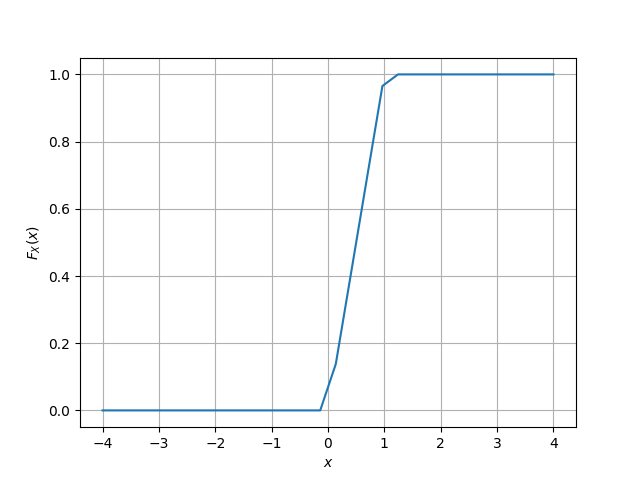
\includegraphics[width=\columnwidth]{U_CDF.png}
\caption{The CDF of $U$}
\label{fig:uni_cdf}
\end{figure}
%
\item
Find a  theoretical expression for $F_{U}(x)$.

\solution

\begin{align}  
f_{U}\brak{x} = 
\begin{cases}
1, & x\in (0,1) \\
0, & \text{otherwise}
\end{cases}
\end{align}
\begin{equation}
    F_U(x) = \int_{-\infty}^{x} f_{U}\brak{x} \,dx  \\
\end{equation}
Hence,
If $ x \leq 0 $,
\begin{align}
    F_U(x) &= \int_{-\infty}^{x} f_{U}\brak{x} \,dx  \\
    F_U(x) &= \int_{-\infty}^{x} 0 \,dx  \\
           &= 0
\end{align}
If $0 <x <1$,
\begin{align}
    F_U(x) &= \int_{0}^{x} f_{U}\brak{x} \,dx  \\
    F_U(x) &= \int_{0}^{x} 1 \,dx  \\
           &= x
\end{align}
If $x \geq 1$,
\begin{align}
    F_U(x) &= \int_{1}^{x} f_{U}\brak{x} \,dx  \\
    F_U(x) &= \int_{1}^{x} 0 \,dx  \\
           &= 0
\end{align}
Hence,
\begin{align}  
F_{U}\brak{x} = 
\begin{cases}
x, & x\in (0,1) \\
0, & \text{otherwise}
\end{cases}
\end{align}
\item
The mean of $U$ is defined as
%
\begin{equation}
E\sbrak{U} = \frac{1}{N}\sum_{i=1}^{N}U_i
\end{equation}
%
and its variance as
%
\begin{equation}
\text{var}\sbrak{U} = E\sbrak{U- E\sbrak{U}}^2 
\end{equation}
Write a C program to  find the mean and variance of $U$.

\solution
\begin{lstlisting}
wget https://github.com/tejalkul/AI1110-Assignments/blob/main/AI1110%20Random%20Variables%20Assignment/codes/mean_variance.c
wget https://github.com/tejalkul/AI1110-Assignments/blob/main/AI1110%20Random%20Variables%20Assignment/codes/coeffs.h
\end{lstlisting}
\begin{align}
    \text{Mean obtained} &= 0.500007 \\
    \text{Variance obtained} &= 0.083301
\end{align}

\item Verify your result theoretically given that

\end{enumerate}
%
\begin{equation}
E\sbrak{U^k} = \int_{-\infty}^{\infty}x^kdF_{U}(x)
\end{equation}
\solution

\begin{align}
    E\sbrak{U^k} &=  0 + \int_{0}^{1} x^k \,dF_{U}\brak{x} + 0 \\
                 &= \frac{1}{k + 1}  \\
    \implies E\sbrak{U} &= \frac{1}{2}\\
                        &= 0.50 \\
             E\sbrak{U^2} &= \frac{1}{3}
\end{align}
Hence,
\begin{align}
    \text{variance} &= E\sbrak{U^2} - \brak{E\sbrak{U}}^2 \\
                    &= \frac{1}{3} - \brak{\frac{1}{2}}^2 \\
                    &= \frac{1}{12} \\
                    &= 0.0833
\end{align}
\section{Central Limit Theorem}
%
\begin{enumerate}[label=\thesection.\arabic*
,ref=\thesection.\theenumi]
%
\item
Generate $10^6$ samples of the random variable
%
\begin{equation}
X = \sum_{i=1}^{12}U_i -6
\end{equation}
%
using a C program, where $U_i, i = 1,2,\dots, 12$ are  a set of independent uniform random variables between 0 and 1
and save in a file called gau.dat
%
\solution

\begin{lstlisting}
wget https://github.com/tejalkul/AI1110-Assignments/blob/main/AI1110%20Random%20Variables%20Assignment/codes/exrand.c
wget https://github.com/tejalkul/AI1110-Assignments/blob/main/AI1110%20Random%20Variables%20Assignment/codes/coeffs.h
\end{lstlisting}
\item
Load gau.dat in python and plot the empirical CDF of $X$ using the samples in gau.dat. What properties does a CDF have?
\\
\solution The CDF of $X$ is plotted in Fig. \ref{fig:gauss_cdf} using code
\begin{lstlisting}
wget https://github.com/tejalkul/AI1110-Assignments/blob/main/AI1110%20Random%20Variables%20Assignment/codes/cdf_plot.py
\end{lstlisting}

\begin{figure}
\centering
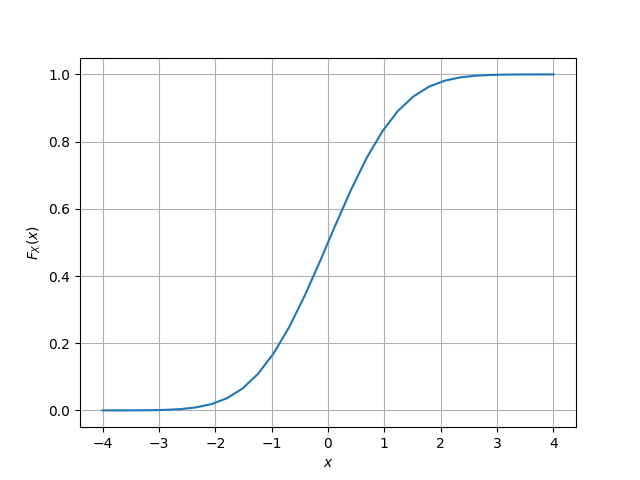
\includegraphics[width=\columnwidth]{X_CDF.png}
\caption{The CDF of $X$}
\label{fig:gauss_cdf}
\end{figure}

The CDF of a random variable U has the following properties:
\begin{enumerate}
    \item $F_{U}\brak{x}$ is a non decreasing function of x where $-\infty < x < \infty$ 
    \item $F_{U}\brak{x}$ ranges from 0 to 1 
    \item $F_{U}\brak{x} = 0$ as $x \rightarrow -\infty$ 
    \item $F_{U}\brak{x} = 1$ as $x \rightarrow \infty$
\end{enumerate}
\item
Load gau.dat in python and plot the empirical PDF of $X$ using the samples in gau.dat. The PDF of $X$ is defined as
\begin{align}
p_{X}(x) = \frac{d}{dx}F_{X}(x)
\end{align}
What properties does the PDF have?
\\
\solution The PDF of $X$ is plotted in Fig. \ref{fig:gauss_pdf} using the code below
\begin{lstlisting}
wget https://github.com/tejalkul/AI1110-Assignments/blob/main/AI1110%20Random%20Variables%20Assignment/codes/pdf_plot.py
\end{lstlisting}
\begin{figure}
\centering
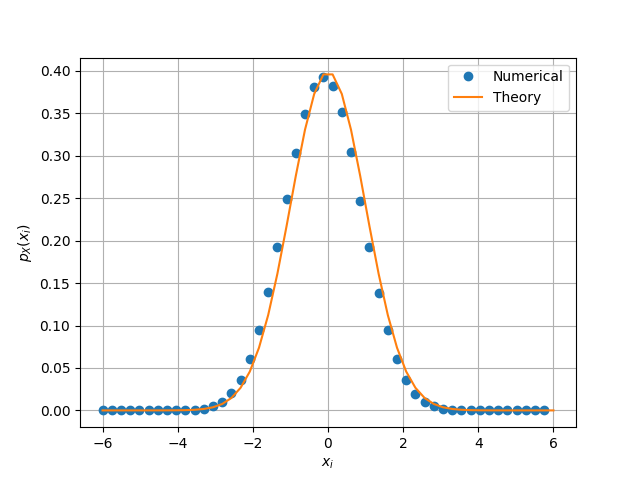
\includegraphics[width=\columnwidth]{X_PDF.png}
\caption{The PDF of $X$}
\label{fig:gauss_pdf}
\end{figure}
The PDF of a random variable X has the following properties:
\begin{enumerate}
    \item The probability density function is non-negative for all the possible values. \\
    \item $ \int_{-\infty}^{\infty} f\brak{x} \,dx  = 1 $ 
    \item $f\brak{x} = 0$ as $x \rightarrow -\infty$
    \item $f\brak{x} = 0$ as $x \rightarrow \infty$
\end{enumerate}
\item Find the mean and variance of $X$ by writing a C program.

\solution
\begin{lstlisting}
wget https://github.com/tejalkul/AI1110-Assignments/blob/main/AI1110%20Random%20Variables%20Assignment/codes/mean_variance.c
wget https://github.com/tejalkul/AI1110-Assignments/blob/main/AI1110%20Random%20Variables%20Assignment/codes/coeffs.h
\end{lstlisting}
\begin{align}
    \text{Mean obtained} &= 0.000326 \\
    \text{Variance obtained} &= 1.000907
\end{align}
\item Given that 
\begin{align}
p_{X}(x) = \frac{1}{\sqrt{2\pi}}\exp\brak{-\frac{x^2}{2}}, -\infty < x < \infty,
\end{align}
repeat the above exercise theoretically.
%
\end{enumerate}
\solution
By definition,
\begin{equation}
    p_{X}\brak{x}dx = dF_{U}\brak{x}
\end{equation}
Hence,
\begin{align}
    E\sbrak{U} &= \int_{-\infty}^{\infty} x p_{X}\brak{x} \,dx \\
               &= \int_{-\infty}^{\infty} x \frac{1}{\sqrt{2\pi}}exp\brak{-\frac{x^2}{2}} \,dx \\
               &= 0
\end{align}
Also,
\begin{equation}
    \text{variance} = E\sbrak{U^2} - \brak{E\sbrak{U}}^2
\end{equation}
\begin{align}
   E\sbrak{U^2} &=  \int_{-\infty}^{\infty} x^2 p_{X}\brak{x} \,dx \\
                &= \int_{-\infty}^{\infty} x^2 \frac{1}{\sqrt{2\pi}}exp\brak{-\frac{x^2}{2}} \,dx \\
                &\text{Using integration by parts,} \\
                &= \int_{-\infty}^{\infty} x x\frac{1}{\sqrt{2\pi}}exp\brak{-\frac{x^2}{2}} \,dx \\
                &= \Big|_{-\infty}^{\infty}-x\frac{1}{\sqrt{2\pi}}e^{\brak{-\frac{x^2}{2}}}  +  \int_{-\infty}^{\infty} \frac{1}{\sqrt{2\pi}}exp\brak{-\frac{x^2}{2}} \\
                &= 0 + \frac{1}{\sqrt{2\pi}}\sqrt{2\pi} \\
                &= 1
    \implies \text{variance} = 1
\end{align}
Also,
\begin{align}
   F_{U}\brak{x} &=  \int_{-\infty}^{x} p_{X}\brak{x} \,dx  \\
                 &= \int_{-\infty}^{x} e^{-\frac{x^2}{2}}\,dx 
\end{align}
\section{From Uniform to Other}
\begin{enumerate}[label=\thesection.\arabic*
,ref=\thesection.\theenumi]
%
\item
Generate samples of 
%
\begin{equation}
V = -2\ln\brak{1-U}
\end{equation}
%
and plot its CDF. 

\solution
\begin{lstlisting}
wget https://github.com/tejalkul/AI1110-Assignments/blob/main/AI1110%20Random%20Variables%20Assignment/codes/exrand.c
wget https://github.com/tejalkul/AI1110-Assignments/blob/main/AI1110%20Random%20Variables%20Assignment/codes/coeffs.h
\end{lstlisting}
The CDF of $X$ is plotted in Fig. \ref{Fig:log_cdf} using the code below
\begin{lstlisting}
wget https://github.com/tejalkul/AI1110-Assignments/blob/main/AI1110%20Random%20Variables%20Assignment/codes/cdf_plot.py
\end{lstlisting}
 
 \item Find a theoretical expression for $F_V(x)$.

\solution
Let, $V = g\brak{U}$
\begin{align}
    V &= -2\ln{(1 - U)} \\
    \implies U &= 1 - e^{-\frac{V}{2}}
\end{align}
Now, 
\begin{align}
    F_{V}\brak{x} &= P\brak{g\brak{U}\leq x} \\
                  &= P\brak{X < g^{-1}\brak{V}} \\
                  &= F_{U}\brak{g^{-1}\brak{V}} \\
                  &= F_{U}\brak{1 - e^{-\frac{V}{2}}}
\end{align}
\begin{align}  
F_{U}\brak{1 - e^{-\frac{V}{2}}} = 
\begin{cases}
1 - e^{-\frac{V}{2}}, & V \in (0,\infty) \\
0, & \text{otherwise}
\end{cases}
\end{align}
\begin{figure}[!ht]
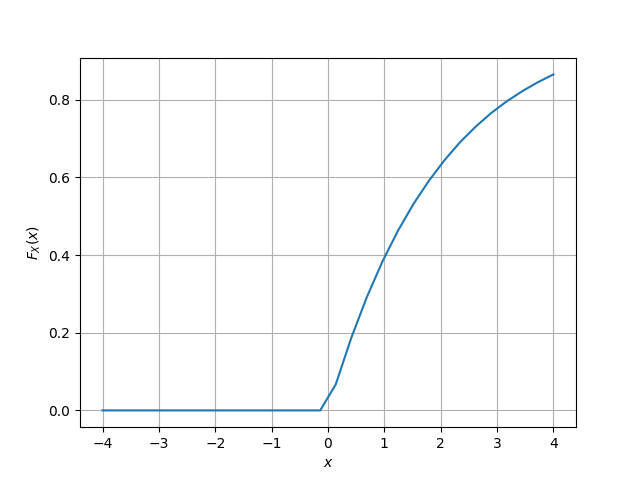
\includegraphics[width = \columnwidth]{V_CDF.png}
\caption{CDF of V}
\label{Fig:log_cdf}
\end{figure}  
%
%\item
%Generate the Rayleigh distribution from Uniform. Verify your result through graphical plots.
\end{enumerate}
\section{Triangular Distribution}
\begin{enumerate}[label=\thesection.\arabic*
,ref=\thesection.\theenumi]
%
\item Generate 
	\begin{align}
		T = U_1+U_2
	\end{align}

\solution
\begin{lstlisting}
wget https://github.com/tejalkul/AI1110-Assignments/blob/main/AI1110%20Random%20Variables%20Assignment/codes/exrand.c
wget https://github.com/tejalkul/AI1110-Assignments/blob/main/AI1110%20Random%20Variables%20Assignment/codes/coeffs.h
\end{lstlisting}
\item Find the CDF of $T$.

\solution
The CDF of T is plotted in Fig. \ref{Fig:tria_exp_cdf} 
\begin{figure}[!ht]
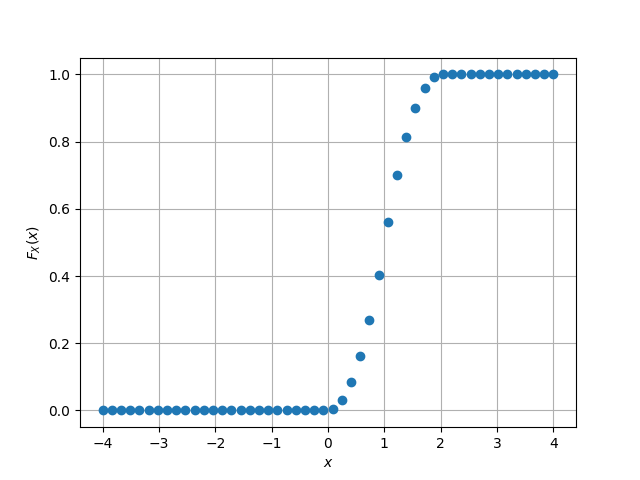
\includegraphics[width = \columnwidth]{T_exp_CDF.png}
\caption{CDF of T}
\label{Fig:tria_exp_cdf}
\end{figure}
\item Find the PDF of $T$.

\solution
The PDF of T is plotted in Fig. \ref{Fig:tria_exp_pdf} 
\begin{figure}[!ht]
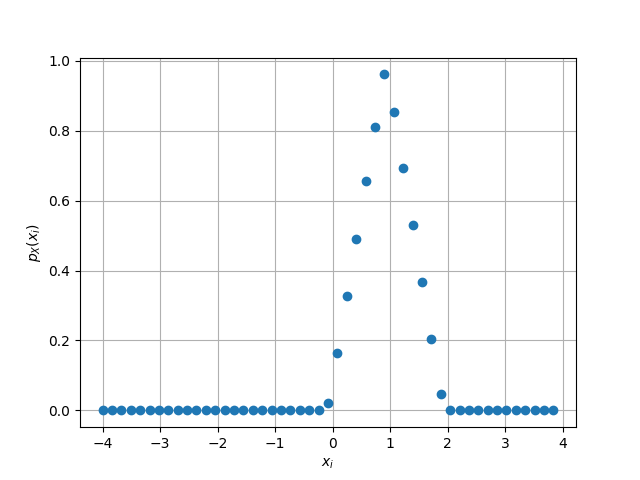
\includegraphics[width = \columnwidth]{T_exp_PDF.png}
\caption{PDF of T}
\label{Fig:tria_exp_pdf}
\end{figure} 
\item Find the theoretical expressions for the PDF and CDF of $T$.

\solution
\begin{align}
    T &= U_1 + U_2 \\
    \implies f_T\brak{T} &= f_{U_1 + U_2}\brak{T} \\
                         &= f_{U_1}\brak{T} * f_{U_2}\brak{T} \\
    &= \int_{-\infty}^{\infty}f_{U_1}\brak{T-U_2}f_{U_2}\brak{U_2}\ dU_2  \label{eq:conv}
\end{align}
since $U_1$ and $U_2$ are independent
Also,
\begin{align}  
f_{U_1}\brak{U_1} = f_{U_2}\brak{U_2} = 
\begin{cases}
1, & x\in (0,1) \\
0, & \text{otherwise}
\end{cases}
\end{align}
Hence for $0 \leq U_2 \leq 1$ , Eq:\eqref{eq:conv} becomes,
\begin{align}
    f_T\brak{T} &= \int_{0}^{1}f_{U_1}\brak{T-U_2}\ dU_2 
\end{align}
If $ 0 \leq T \leq 1 $,
\begin{align}
    f_T(T) &= \int_{0}^{T} \,dU_2  \\
           &= T
\end{align}
If $1 < T \leq 2 $,
\begin{align}
    f_T(T) &= \int_{T-1}^{1} \,dU_2  \\
           &= 2 - T
\end{align}
\begin{align}  
f_{T}\brak{T} = 
\begin{cases}
T, & 0 \leq T \leq 1 \\
2 - T, & 1 < T \leq 2 \\
0, & \text{otherwise}
\end{cases}
\end{align}
Now,
\begin{equation}
    F_T(T) = \int_{-\infty}^{T} f_{T}\brak{T} \,dT  \\
\end{equation}
Hence, if $ T < 0 $,
\begin{align}
    F_T(T) &= \int_{-\infty}^{T} f_{T}\brak{T}\,dT  \\
           &= \int_{-\infty}^{T} 0\,dT  \\
           &= 0
\end{align}
If $ 0 \leq T \leq 1 $,
\begin{align}
    F_T(T) &= \int_{0}^{T} f_{T}\brak{T}\,dT  \\
           &= \int_{0}^{T} T\,dT  \\
           &= \frac{T^2}{2}
\end{align}
If $1 < T \leq 2 $,
\begin{align}
    F_T(T) &= \int_{0}^{1} f_{T}\brak{T}\,dT  + \int_{1}^{T} f_{T}\brak{T}\,dT  \\
           &= \int_{0}^{1} T\,dT  + \int_{1}^{T} (2 - T)\,dT  \\
           &= \frac{1}{2} + \frac{4T - T^2 - 3}{2} \\
           &= 1 - \frac{(2-T)^2}{2}
\end{align}
If $ T > 2 $,
\begin{align}
    F_T(T) &= \int_{2}^{T} f_{T}\brak{T}\,dT  \\
           &= \int_{2}^{T} 0\,dT  \\
           &= 0
\end{align}
\begin{align}  
F_{T}\brak{T} = 
\begin{cases}
\frac{T^2}{2}, & 0 \leq T \leq 1 \\
1 - \frac{(2-T)^2}{2}, & 1 < T \leq 2 \\
0, & \text{otherwise}
\end{cases}
\end{align}
\item Verify your results through a plot. 

\solution
The CDF of T is plotted in Fig. \ref{Fig:tria_cdf} below 
\begin{figure}[!ht]
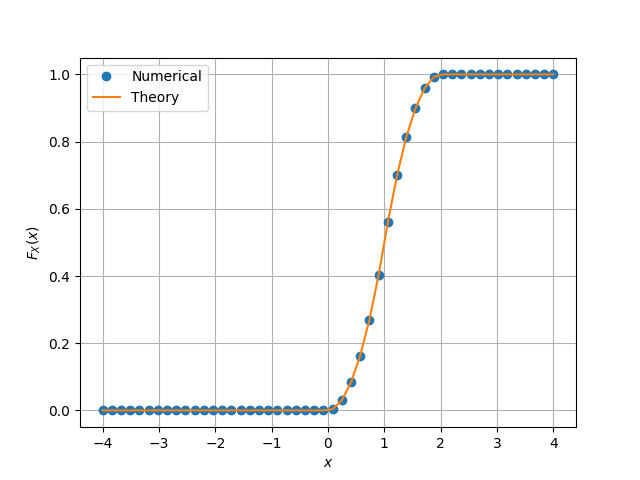
\includegraphics[width = \columnwidth]{T_CDF.png}
\caption{CDF of T}
\label{Fig:tria_cdf}
\end{figure}

The PDF of T is plotted in Fig. \ref{Fig:tria_pdf} below 
\begin{figure}[!ht]
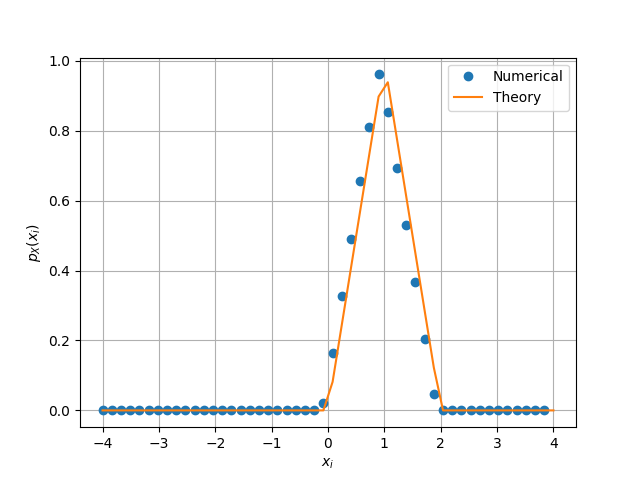
\includegraphics[width = \columnwidth]{T_PDF.png}
\caption{PDF of T}
\label{Fig:tria_pdf}
\end{figure} 

Using codes
\begin{lstlisting}
wget https://github.com/tejalkul/AI1110-Assignments/blob/main/AI1110%20Random%20Variables%20Assignment/codes/cdf_plot.py
wget https://github.com/tejalkul/AI1110-Assignments/blob/main/AI1110%20Random%20Variables%20Assignment/codes/pdf_plot.py
\end{lstlisting}
\end{enumerate}
\section{Maximul Likelihood}
\begin{enumerate}[label=\thesection.\arabic*
,ref=\thesection.\theenumi]
\item Generate equiprobable $X \in \cbrak{1,-1}$.

\solution
\begin{lstlisting}
wget https://github.com/tejalkul/AI1110-Assignments/blob/main/AI1110%20Random%20Variables%20Assignment/codes/exrand.c
wget https://github.com/tejalkul/AI1110-Assignments/blob/main/AI1110%20Random%20Variables%20Assignment/codes/coeffs.h
\end{lstlisting}
\item Generate 
\begin{equation}
Y = AX+N,
\end{equation}
		where $A = 5$ dB,  and $N \sim \gauss{0}{1}$.

\solution
\begin{lstlisting}
wget https://github.com/tejalkul/AI1110-Assignments/blob/main/AI1110%20Random%20Variables%20Assignment/codes/exrand.c
wget https://github.com/tejalkul/AI1110-Assignments/blob/main/AI1110%20Random%20Variables%20Assignment/codes/coeffs.h
\end{lstlisting}
	\item Plot $Y$ using a scatter plot.
The scatter plot of Y is plotted in Fig. \ref{Fig:Y_scatter} below 

\solution
\begin{figure}[!ht]
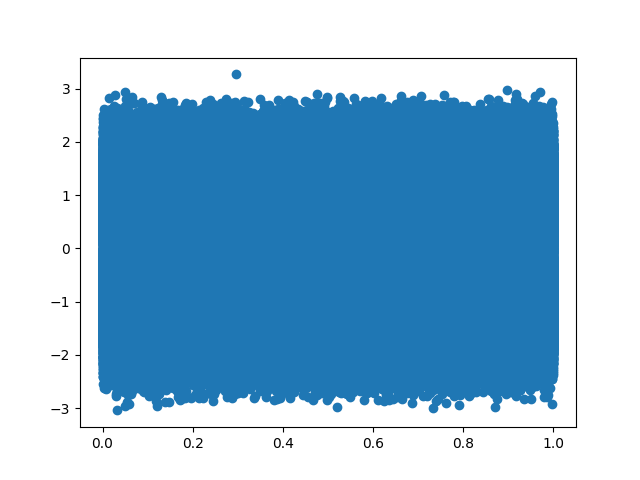
\includegraphics[width = \columnwidth]{Y_scatter.png}
\caption{Scatter plot of Y}
\label{Fig:Y_scatter}
\end{figure} 

	\item Guess how to estimate $X$ from $Y$.
	
	\solution
	
	To estimate X from Y we define the following function,
	\begin{align}  
g\brak{y} = 
\begin{cases}
1, & y \in (0,\infty)\\
-1 & y \in (-\infty,0] \\
\end{cases}
\end{align}
Hence using this function we can operate on Y to find X
\item
\label{ml-ch4_sim}
Find 
\begin{equation}
	P_{e|0} = \pr{\hat{X} = -1|X=1}
\end{equation}
and 
\begin{equation}
	P_{e|1} = \pr{\hat{X} = 1|X=-1}
\end{equation}

\solution
\begin{lstlisting}
wget https://github.com/tejalkul/AI1110-Assignments/blob/main/AI1110%20Random%20Variables%20Assignment/codes/exrand.c
wget https://github.com/tejalkul/AI1110-Assignments/blob/main/AI1110%20Random%20Variables%20Assignment/codes/coeffs.h
\end{lstlisting}
Values obtained
\begin{align}
    P_{e|0} &= 0.311084 \\
    P_{e|1} &= 0.311586
\end{align}
%
\item Find $P_e$ assuming that $X$ has equiprobable symbols.

\solution
We have,
\begin{align}
    P_{e|0} &= \pr{\hat{X} = -1|X=1} \\
            &= \pr{AX + N < 0|X=1} \\    
            &= \pr{N < -A} \\
            &= \int_{-\infty}^{-A} \frac{1}{\sqrt{2\pi}}e^{-x^2/2}\,dx  \\
            &= \int_{A}^{\infty} \frac{1}{\sqrt{2\pi}}e^{-x^2/2}\,dx  \\
            &= Q_{N}\brak{A}
\end{align}
%
\begin{align}
    P_{e|1} &= \pr{\hat{X} = 1|X=-1} \\
            &= \pr{AX + N > 0|X=-1} \\    
            &= \pr{N > A} \\
            &= Q_{N}\brak{A}
\end{align}
%
\begin{align}
    P_e &= P_{e|0}P\brak{X = 1} + P_{e|1}P\brak{X = -1} \\
        &= P_{e|0}\frac{1}{2} + P_{e|1}\frac{1}{2} \\
        &= Q_{N}\brak{A}\frac{1}{2} + Q_{N}\brak{A}\frac{1}{2} \\
        &= Q_{N}\brak{A}
\end{align}
\item
Verify by plotting  the theoretical $P_e$ with respect to $A$ from 0 to 10 dB.

\solution
\begin{figure}[!ht]
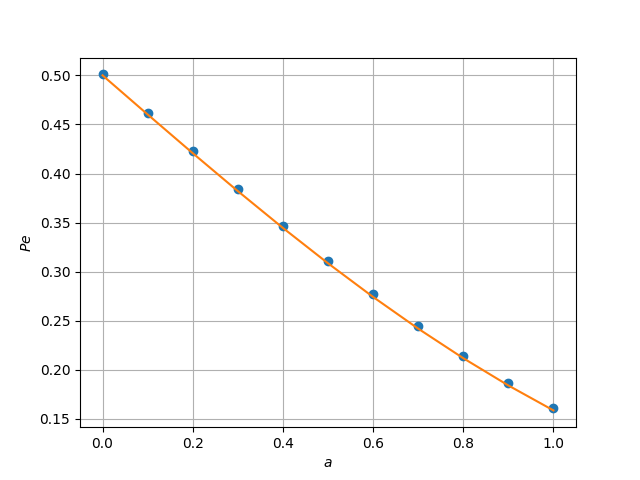
\includegraphics[width = \columnwidth]{P_err.png}
\caption{$P_e vs A$}
\label{Fig:P_e}
\end{figure} 
%
\item Now, consider a threshold $\delta$  while estimating $X$ from $Y$. Find the value of $\delta$ that minimizes the theoretical $P_e$.
To estimate X from Y we now define the following function,
	\begin{align}  
g\brak{y} = 
\begin{cases}
1, & y \in (\delta,\infty)\\
-1 & y \in (-\infty,\delta] \\
\end{cases}
\end{align}
We have,
\begin{align}
    P_{e|0} &= \pr{\hat{X} = -1|X=1} \\
            &= \pr{AX + N < \delta|X=1} \\    
            &= \pr{N < \delta - A} \\
            &= \int_{-\infty}^{\delta - A} \frac{1}{\sqrt{2\pi}}e^{-x^2/2}\,dx  \\
            &= \int_{A - \delta}^{\infty} \frac{1}{\sqrt{2\pi}}e^{-x^2/2}\,dx  \\
            &= Q_{N}\brak{A - \delta}
\end{align}
%
\begin{align}
    P_{e|1} &= \pr{\hat{X} = 1|X=-1} \\
            &= \pr{AX + N > \delta|X=-1} \\    
            &= \pr{N > \delta + A} \\
            &= Q_{N}\brak{\delta + A}
\end{align}
Hence,
\begin{align}
    P_e &= P_{e|0}P\brak{X = 1} + P_{e|1}P\brak{X = -1} \\
        &= P_{e|0}\frac{1}{2} + P_{e|1}\frac{1}{2} \\
        &= Q_{N}\brak{A - \delta}\frac{1}{2} + Q_{N}\brak{A + \delta}\frac{1}{2} 
\end{align}
To minimize $P_e$  we differentiate $P_e$ wrt $\delta$,
\begin{align}
0 &= \frac{d}{d\delta} \left(\frac{1}{2}(Q_N(A - \delta) + Q_N(A + \delta))\right) \\
&= \frac{1}{2} \brak{\frac{1}{\sqrt{2\pi}} e^{-\frac{(\delta - A)^2}{2}} - \frac{1}{\sqrt{2\pi}} e^{-\frac{(A + \delta)^2}{2}} } \\
\end{align}
Therefore,
\begin{align}
    (\delta - A)^2 &= (A + \delta)^2 \\
    \implies \delta &= 0 
\end{align}

\item Repeat the above exercise when 
	\begin{align}
		p_{X}(0) = p
	\end{align}
	
	\solution
	Let $P{X = -1}$ = p, hence $P{X = 1} = 1-p $
	Hence,
	\begin{align}
	    P_e &= P_{e|0}P\brak{X = 1} + P_{e|1}P\brak{X = -1} \\
	    P_e &= P_{e|0}(1-p) + P_{e|1}p \\
	        &= Q_{N}\brak{A - \delta}(1-p) + Q_{N}\brak{A + \delta}p
	 \end{align}
Differentiating like before,
\begin{equation}
0 &= p \frac{1}{\sqrt{2\pi}} e^{-\frac{(\delta - A)^2}{2}} - (1-p)\frac{1}{\sqrt{2\pi}} e^{-\frac{(A + \delta)^2}{2}}  
\end{equation}
Taking log,
\begin{align}
\ln{p} - \frac{(\delta - A)^2}{2} &= \ln{(1-p)} + \frac{(\delta + A)^2}{2} \\
    \implies \delta &= \frac{1}{2A} \ln{\frac{1-p}{p}}
\end{align}
	
\item Repeat the above exercise using the MAP criterion.
		\end{enumerate}
\section{Gaussian to Other}
\begin{enumerate}[label=\thesection.\arabic*
,ref=\thesection.\theenumi]
\item
Let $X_1 \sim  \gauss{0}{1}$ and $X_2 \sim  \gauss{0}{1}$. Plot the CDF and PDF of
%
\begin{equation}
V = X_1^2 + X_2^2
\end{equation}

\solution
Data for the plots is generated using
\begin{lstlisting}
wget https://github.com/tejalkul/AI1110-Assignments/blob/main/AI1110%20Random%20Variables%20Assignment/codes/exrand.c
wget https://github.com/tejalkul/AI1110-Assignments/blob/main/AI1110%20Random%20Variables%20Assignment/codes/coeffs.h
\end{lstlisting}
The CDF of V is plotted in Fig. \ref{Fig:chi_cdf} 
\begin{figure}[!ht]
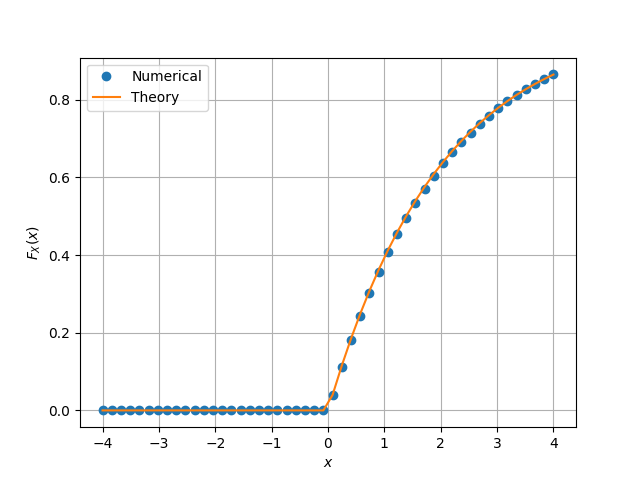
\includegraphics[width = \columnwidth]{V2_CDF.png}
\caption{CDF of V}
\label{Fig:chi_cdf}
\end{figure}

The PDF of V is plotted in Fig. \ref{Fig:chi_pdf} 

\begin{figure}[!ht]
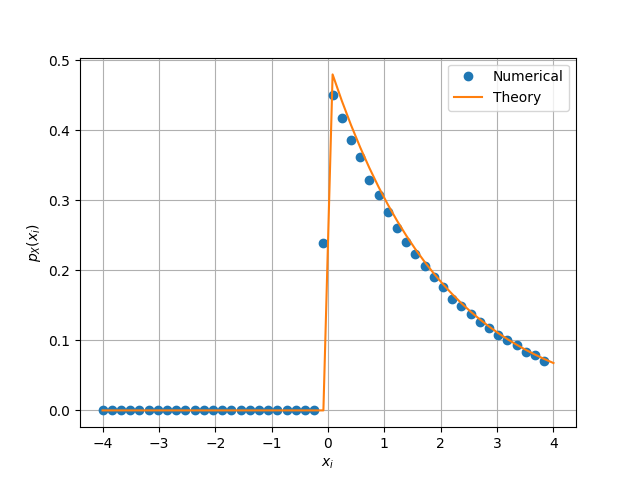
\includegraphics[width = \columnwidth]{V2_PDF.png}
\caption{PDF of V}
\label{Fig:chi_pdf}
\end{figure} 

Using codes
\begin{lstlisting}
wget https://github.com/tejalkul/AI1110-Assignments/blob/main/AI1110%20Random%20Variables%20Assignment/codes/cdf_plot.py
wget https://github.com/tejalkul/AI1110-Assignments/blob/main/AI1110%20Random%20Variables%20Assignment/codes/pdf_plot.py
\end{lstlisting}
%
%
%
\item
If
%
\begin{equation}
F_{V}(x) = 
\begin{cases}
1 - e^{-\alpha x} & x \geq 0 \\
0 & x < 0,
\end{cases}
\end{equation}
%
find $\alpha$.
%

\solution
$X_1$ and $X_2$ are i.i.d . Let,
\begin{align}
    X_1 &= R\cos{\theta} \\
    X_2 &= R\sin{\theta}
\end{align}
Using Jacobian transform we have,
\begin{align}
   f_{X_1X_2}\brak{X_1,X_2} = \frac{1}{|J\brak{R,\theta}|} f_{R\theta}\brak{R,\theta}
\end{align}
Now,Jacobian matrix is given as follows,
\begin{align}
    J                        & = \myvec{\frac{\delta x_1}{\delta R}                      & \frac{\delta x_1}{\delta \theta} \\ \frac{\delta x_2}{\delta R} & \frac{\delta x_2}{\delta \theta}}\\
    J                        & = \myvec{\cos\theta                                       & -R\sin\theta                     \\ \sin\theta & R\cos\theta}\\
    |J|                      & = R \\
    \implies f_{X_1X_2}\brak{X_1,X_2} &= \frac{1}{R}f_{R\theta}\brak{R,\theta}
\end{align}
Now,
\begin{align}
    f_{X_1X_2}\brak{X_1,X_2} &= f_{X_1}\brak{X_1}f_{X_2}\brak{X_2} \\
                             &= \frac{1}{\sqrt{2\pi}}e^{\frac{-X_1^2}{2}} \frac{1}{\sqrt{2\pi}}e^{\frac{-X_2^2}{2}} \\
                             &= \frac{1}{2\pi}e^{\frac{-\brak{X_1^2 + X_2^2}}{2}} \\
                             &= \frac{1}{2\pi}e^{\frac{-R^2}{2}}
\end{align}
Hence,
\begin{align}
    f_{R\theta}\brak{R,\theta} &= \frac{R}{2\pi}e^{\frac{-R^2}{2}} \\
    \implies f_{R}\brak{R} &= \int_{0}^{2\pi} \frac{R}{2\pi}e^{\frac{-R^2}{2}}\,d\theta \\
                           &= R e^{\frac{-R^2}{2}}
\end{align}
Hence,
\begin{equation}
f_{R}(R) = 
\begin{cases}
R e^{\frac{-R^2}{2}} & x \geq 0 \\
0 & x < 0,
\end{cases}
\end{equation}
\begin{equation}
F_{R}(R) = 
\begin{cases}
1 - e^{\frac{-R^2}{2}} & x \geq 0 \\
0 & x < 0,
\end{cases}
\end{equation}
Now, 
\begin{align}
  F_{V}\brak{x} &= P\brak{V \leq x} \\
                &= P\brak{R^2 \leq x} \\
                &= P\brak{R \leq \sqrt{x}} \\
                &= F_{R}\brak{\sqrt{x}} 
\end{align}
Hence,
\begin{equation}
F_{V}(x) = 
\begin{cases}
1 - e^{\frac{-x}{2}} & x \geq 0 \\
0 & x < 0,
\end{cases}
\end{equation}
\begin{equation}
    \implies \alpha = \frac{1}{2}
\end{equation}



\item
\label{ch3_raleigh_sim}
Plot the CDF and PDf of
%
\begin{equation}
A = \sqrt{V}
\end{equation}
%
\solution
Data for the plots is generated using
\begin{lstlisting}
wget https://github.com/tejalkul/AI1110-Assignments/blob/main/AI1110%20Random%20Variables%20Assignment/codes/exrand.c
wget https://github.com/tejalkul/AI1110-Assignments/blob/main/AI1110%20Random%20Variables%20Assignment/codes/coeffs.h
\end{lstlisting}
The CDF of A is plotted in Fig. \ref{Fig:root_V_cdf} below 
\begin{figure}[!ht]
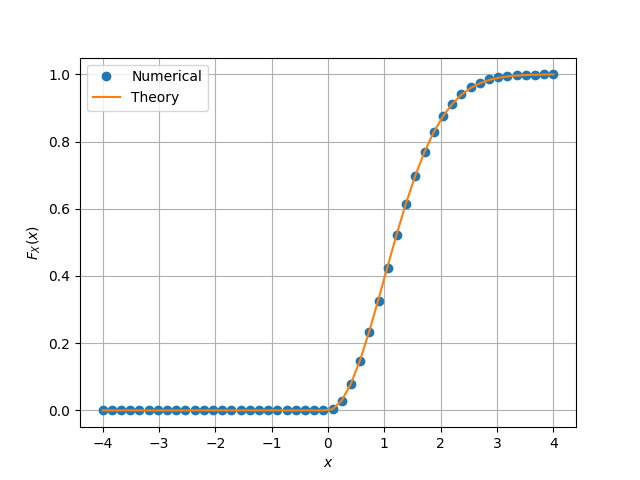
\includegraphics[width = \columnwidth]{A_CDF.png}
\caption{CDF of A}
\label{Fig:root_V_cdf}
\end{figure}

The PDF of A is plotted in Fig. \ref{Fig:root_V_pdf} below 
\begin{figure}[!ht]
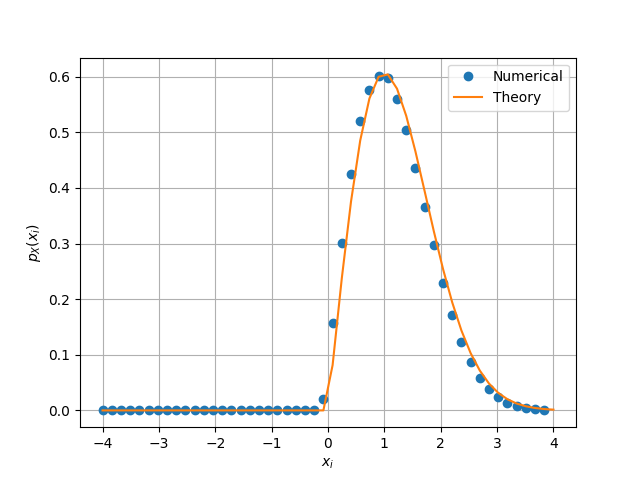
\includegraphics[width = \columnwidth]{A_PDF.png}
\caption{PDF of A}
\label{Fig:root_V_pdf}
\end{figure} 

Using codes
\begin{lstlisting}
wget https://github.com/tejalkul/AI1110-Assignments/blob/main/AI1110%20Random%20Variables%20Assignment/codes/cdf_plot.py
wget https://github.com/tejalkul/AI1110-Assignments/blob/main/AI1110%20Random%20Variables%20Assignment/codes/pdf_plot.py
\end{lstlisting}
\end{enumerate}
\section{Conditional Probability}
\begin{enumerate}[label=\thesection.\arabic*
,ref=\thesection.\theenumi]
\item
\item
\label{ch4_sim}
Plot 
\begin{equation}
P_e = \pr{\hat{X} = -1|X=1}
\end{equation}
%
for 
\begin{equation}
Y = AX+N,
\end{equation}
where $A$ is Raleigh with $E\sbrak{A^2} = \gamma, N \sim \gauss{0}{1}, X \in \brak{-1,1}$ for $0 \le \gamma \le 10$ dB.
%
\item
Assuming that $N$ is a constant, find an expression for $P_e$.  Call this $P_e(N)$
%
\item
%
\label{ch4_anal}
For a function $g$,
\begin{equation}
E\sbrak{g(X)} = \int_{-\infty}^{\infty}g(x)p_{X}(x)\, dx
\end{equation}
%
Find $P_e = E\sbrak{P_e(N)}$.
%
\item
Plot $P_e$ in problems \ref{ch4_sim} and \ref{ch4_anal} on the same graph w.r.t $\gamma$.  Comment.
		\end{enumerate}
\section{Two Dimensions}
Let 
\begin{equation}
\mbf{y} = A\mbf{x} + \mbf{n},
\end{equation}
where 
\begin{align}
x &\in \brak{\mbf{s}_0,\mbf{s}_1}, 
\mbf{s}_0 = 
\begin{pmatrix}
1 
\\
0
\end{pmatrix},
\mbf{s}_1 = 
\begin{pmatrix}
0 
\\
1
\end{pmatrix}
\\
\mbf{n} &= 
\begin{pmatrix}
n_1
\\
n_2
\end{pmatrix},
n_1,n_2 \sim \gauss{0}{1}.
\end{align}
%
\begin{enumerate}[label=\thesection.\arabic*
,ref=\thesection.\theenumi]
%%
\item
\label{ch5_fsk}
Plot 
%
\begin{equation}
\mbf{y}|\mbf{s}_0 \text{ and } \mbf{y}|\mbf{s}_1
\end{equation}
%
on the same graph using a scatter plot.
%
\item
For the above problem, find a decision rule for detecting the symbols $\mbf{s}_0 $ and $\mbf{s}_1$.
%
\item
Plot 
\begin{equation} 
P_e = \pr{\hat{\mbf{x}} = \mbf{s}_1|\mbf{x} = \mbf{s}_0}
\end{equation}
with respect to the SNR from 0 to 10 dB.
%
\item
Obtain an expression for $P_e$. Verify this by comparing the theory and simulation plots on the same graph.
%
		\end{enumerate}
\end{document}
